\documentclass[10pt,conference,compsocconf]{IEEEtran}

\usepackage{hyperref}
\usepackage{graphicx}	% For figure environment
\usepackage{amsmath}
%%%%%%%%%%%%%%%%%%%%%%%%%%%%%%%%%%%%%%%%%%%%%%%%%%%%%%%%%%%%%
% Some tools
% Includes a figure
% The first parameter is the label, which is also the name of the figure
%   with or without the extension (e.g., .eps, .fig, .png, .gif, etc.)
%   IF NO EXTENSION IS GIVEN, LaTeX will look for the most appropriate one.
%   This means that if a DVI (or PS) is being produced, it will look for
%   an eps. If a PDF is being produced, it will look for nearly anything
%   else (gif, jpg, png, et cetera). Because of this, when I generate figures
%   I typically generate an eps and a png to allow me the most flexibility
%   when rendering my document.
% The second parameter is the width of the figure normalized to column width
%   (e.g. 0.5 for half a column, 0.75 for 75% of the column)
% The third parameter is the caption.
\newcommand{\scalefig}[4]{
  \begin{figure}[ht!]
    % Requires \usepackage{graphicx}
    \centering
    \includegraphics[width=#2\columnwidth]{pics/#1}
 \caption{#3}
    \label{#4}
  \end{figure}}
  
  \newcommand{\doublefig}[5]{
  \begin{figure}[ht!]
    % Requires \usepackage{graphicx}
    \centering
    \includegraphics[width=#3\columnwidth]{../pics/#1}\hfill
    \includegraphics[width=#3\columnwidth]{../pics/#2}
 \caption{#4}
    \label{#5}
  \end{figure}}

% \mathbf
\newcommand{\m}[1]{\mathbf{#1}}
\newcommand{\xx}{\mathbf{x}}
\newcommand{\xt}{\mathbf{x}^T}
\newcommand{\yy}{\mathbf{y}}
\newcommand{\ww}{\mathbf{w}}
\newcommand{\XX}{\mathbf{X}}
 
\newcommand{\Lagr}{\mathcal{L}}
\newcommand{\Lmse}{\Lagr_{MSE}}

% argmin
\newcommand{\argmin}[1]{\underset{#1}{\operatorname{argmin}}}
\newcommand{\argmax}[1]{\underset{#1}{\operatorname{argmax}}}
\newcommand{\mmin}[1]{\underset{#1}{\operatorname{min}}}
\newcommand{\mmax}[1]{\underset{#1}{\operatorname{max}}}

\newcommand*\colvec[3][]{
    \begin{pmatrix}\ifx\relax#1\relax\else#1\\\fi#2\\#3\end{pmatrix}
}


\begin{document}
\title{Project 2: Road Segmentation}

\author{
  Team Bazinga:
  Gael Moccand, Pascal Bienz\\
  gael.moccand@gmail.com, pascal.bienz@gmail.com\\
  \textit{Machine Learning Course, EPFL}
}

\maketitle

\begin{abstract}

\end{abstract}

\section{Introduction}
bla bla (Pascal)
\subsection{Data}
General description of images
100 images + gt 
->not enough to train and avoid overfitting + rotation to have roads in every direction (5, 10,...355 degrees)
from image to linear vector
patchs + moyenne/variance + hog (do sqrt with hitogram -> see kiko)
gt to label (25\% -> 191)
neural nets -> resize to 224x224

Training vs Validation = 80/20
(Gael)

\section{Methodology}
1. BER (pascal)
2. feats = mean + var / patch + hog
   method = logistic reg
   + sqrt ? 
   (pascal)
   
3. NN -> segnet, segnet connected, segnet connected gate
   graph with epochs -> loss vs epoch
   (Gael)


\section{Results}
...

\section{Discussion}

%There are few things that can probably be improved in order to get better prediction. Firstly MSE is not a good cost function when outliers are present which is the case here. One should thus look for another cost function. Then, least squares is a pretty basic model. The next step would be to use a logistic regression instead. However, we could not manage to make it converge.\\
%Regarding preprocessing, an improvement would be to weight the features independently instead of having them equally weighted. Moreover, there is a feature which only has integer numbers. A possible improvement would be not to feed it to the polynomial basis and use this feature directly. Unfortunately, this trick has not shown much improvement on the final score. Finally, when the preprocessing changed from simple to complex, the whole optimization process should be done again to guarantee the best prediction with the appropriate hyperparameters.

\section{Summary}
In this work we have shown that one can have a fairly good prediction using simple machine learning techniques like the least squares regression and the ridge regularization as long as one takes care of handling the data properly. We have also highlighted the fact that in the field of machine learning, one should be careful and that some intuition that seem good a priori yield worse prediction.%

%\begin{figure}[tbp]
%  \centering
%  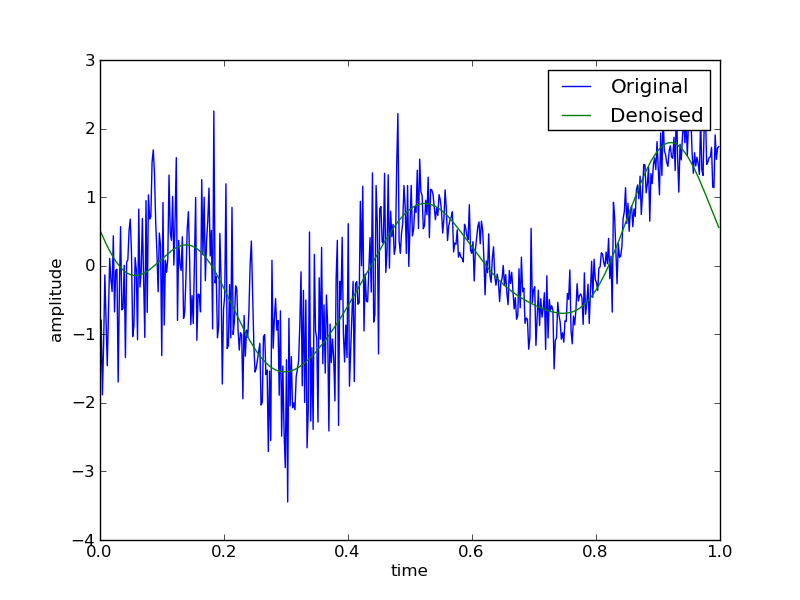
\includegraphics[width=\columnwidth]{denoised_signal_1d}
%  \caption{Signal compression and denoising using the Fourier basis.}
%  \vspace{-3mm}
%  \label{fig:denoise-fourier}
%\end{figure}
%\begin{figure}[htbp]
%  \centering
%  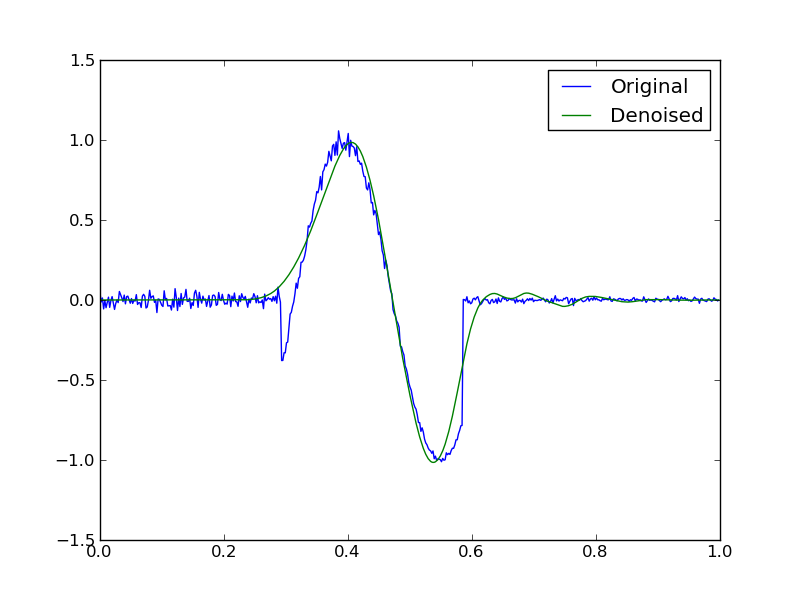
\includegraphics[width=\columnwidth]{local_wdenoised_1d}
%  \vspace{-3mm}
%  \caption{Signal compression and denoising using the Daubechies wavelet basis.}
%  \label{fig:denoise-wavelet}
%\end{figure}


%\begin{table*}[htbp]
%  \centering
%  \begin{tabular}[c]{|l||l|l|l|}
%    \hline
%    Basis&Support&Suitable signals&Unsuitable signals\\
%    \hline
%    Fourier&global&sine like&localized\\
%    wavelet&local&localized&sine like\\
%    \hline
%  \end{tabular}
%  \caption{Characteristics of Fourier and wavelet basis.}
%  \label{tab:fourier-wavelet}
%\end{table*}
%
%
%\begin{table} [htbp]
%  \centering
%  \begin{tabular}[c]{|l|l|}
%    \hline
%    Method & Test error\\
%    \hline
%    Simple preproc. + LS + $M=2$ &0.8019\\
%    Simple preproc. + LS + Ridge & 0.8252\\
%    Complex preproc. + LS + Ridge $M=8$ & \textbf{0.7467}\\
%    \hline
%  \end{tabular}
%  \caption{Test errors of different prediction methods.}
%  \label{tab:results}
%\end{table}

%\section*{Acknowledgements}
%The author thanks Christian Sigg for his careful reading and helpful
%suggestions.

\bibliographystyle{IEEEtran}
\bibliography{literature}

\end{document}
